\section{Recursion}
\label{sec:recursion}

Recursion is the process of repeating items in a self-similar way. It
is a concept that appears often in computer science and other branches
of mathematics (e.g.~number theory, fractals), but it has also
attracted some interest from fields like the arts in recent times
(look up ``recursive images'' on your favourite search engine). 

In programming, the most basic form of recursion happens when a method
calls itself. This can be done in any modern programming language, and
definitely in Java. We have already seen some examples of recursive
calls, e.g.~when we tried to calculate the depth of a tree: 

\begin{verbatim}
    // Method of class Node/Tree
    public int depth() {
        int leftDepth = 0;
        if (left != null) {
            leftDepth = left.depth();
        }
        int rightDepth = 0;
        if (right != null) {
            rightDepth = right.depth();
        }
        int depthBelow = Math.max(leftDepth, rightDepth);
        return 1 + depthBelow;
    }
\end{verbatim}

This method calls itself twice before it can return a value to the
caller. In order to return the depth under a node in a binary tree,
the depth under the left branch is calculated (if it exists, otherwise
it is zero), then the depth under the right branch, and then the
result is the maximum of both depths plus one. The method
\verb+depth()+ is \emph{recursive}. 

In this section we are going to
learn more about how recursion works, when it is a good idea to use
it, and what are the possible pitfalls and how to avoid them. 

\paragraph{Classical examples: factorials and Fibonacci numbers}
\label{sec:class-exampl-fact}

The factorial of a natural number is represented with an exclamation
mark (!) and defined\footnote{If you like maths and would like to see
  how the factorial of a \emph{real} number is defined, search for the
  $\Gamma$ (gamma) function.} as:  

$$ n! = n \cdot (n - 1) \cdot (n - 2) \cdot \ldots 2 \cdot 1 $$

This definition makes it very easy to write a function that calculates
the factorial of a number recursively: 

\begin{verbatim}
    public static int factorial(int n) {
        if (n == 1) {
          return 1; 
        } else {
            int result = n * factorial(n-1);
            return result;
        }
    }
\end{verbatim}

(Note that the method is static because it has no side effects,
i.e.~it is a pure function). 

If the argument is 1, the function returns 1 (because 1! =
1). Otherwise, the function returns the argument multiplied by the
factorial of the argument minus one; that function call will in turn
return its argument (n-1) multiplied by the factorial of its argument
minus one (n-2); and so on. If we want to calculate the factorial
of~4, the resulting calculations look like this: 

$$ factorial(4) = 4 \cdot factorial(3) = 
   4 \cdot (3 \cdot factorial(2)) = 
   4 \cdot (3 \cdot (2 \cdot factorial(1))) = $$ 

$$ = 4 \cdot (3 \cdot (2 \cdot 1)) = 4 \cdot (3 \cdot 2) = 4 \cdot 6 = 24 $$

Another classical example of recursivity are Fibonacci
numbers\footnote{Fibonacci numbers were discovered by Italian mathematician
Leonardo di Pisa (known as Fibonacci) in the early 13$^{th}$ century
as an ideal solution to the growth of the population of rabbits. The
sequence of Fibonacci number starts as 1, 1, 2, 3, 5, 8, 13, 21, 34,
55, 89\ldots Fibonacci introduced arabic numerals to the West, and
thanks to him we can write 2989 instead of MMCMLXXXVIII.}.
Fibonacci numbers are defined recursively as:

$$ F(1) = F(2) = 1 $$

$$ F(n) = F(n-1) + F(n-2) $$

and have many applications in computer science and biology, among
other fields. As they are defined recursively, a recursive method to
calculate the n$^{th}$ Fibonacci number is quite straightforward to
write: 

\begin{verbatim}
    public static int fib(int n) {
        if ((n == 1) || (n == 2)) {
          return 1; 
        } else {
            int result = fib(n-1) + fib(n-2);
            return result;
        }
    }
\end{verbatim}

\subsection{How does recursion work?}
\label{sec:how-does-recursion}

Recursion works as any other method call. There is no magic. 

When a statement in Java calls a method, the same process is always
followed: 

\begin{enumerate}
\item A new level is added to the stack.
\item The values given by the caller code are copied into the
  parameters in the new level.
\item A hidden parameter ``this'' is also copied into the stack,
  pointing to the object where the method is called.
\item The code of the method is executed as usual. Any new local
  variable is created on the new level in the stack. 
\item When a \verb+return+ statement is reached, the corresponding
  return value (if any) is stored.
\item The level in the stack is wiped out, and its local variables
  (and parameter values) forgotten. The return value (if any) is
  returned to the original caller code (and usually assigned to a
  variable).
\end{enumerate}

This does not change in the case of a recursive call. If we take the
calculation of 4! before as an example, the computer stack changes are
represented if Figure~\ref{fig:fact}. First, a level is added to the
stack and the parameters are copied (only \verb+n+ in this case, with
value~4). The code of the method is executed line by line: as \verb+n+
is not 
equal to~1, a new local variable \verb+result+ is created; its value
is~1 plus the result of calling a method. A new level is added to the
stack, and the parameter values are copied (only \verb+n+ again, but
this time with value~3). A local variable \verb+result+ is created and
then the method is called again so we need to add a new level in the
stack. The process is repeated once more, and we call the method with
a value of 1 for \verb+n+. At this point, the method returns 1. Then
the calling method can finally calculate the value of \verb+result+,
which is $2 \cdot 1 = 2$, and returns it. Then the calling method can
calculate \verb+result+ itself, which in this case is $3 \cdot 2 = 6$,
and return it. The calling method can then find the value of
\verb+result+ (24) and return it. 

As you can see, a method recursively calling itself is no different
from a method calling another method. For every method call, recursive
or not, the calling code remains \emph{on pause} while the new level
in the stack is created and the code of the called method is
executed (in the example, the value is result is not defined until a
return value is received from the called method). 
When a result is returned, the calling code can continue its
execution. When a method calls a method that calls a method, etc,
several levels are added to the stack, and several methods are waiting
for a return value. Recursive calls are exactly the same, the only
difference being that the same code is executed over and over again
\emph{but on different levels of the stack}, which means that local
variables are new and independent. 

\begin{figure}[hbtp]
  \centering
  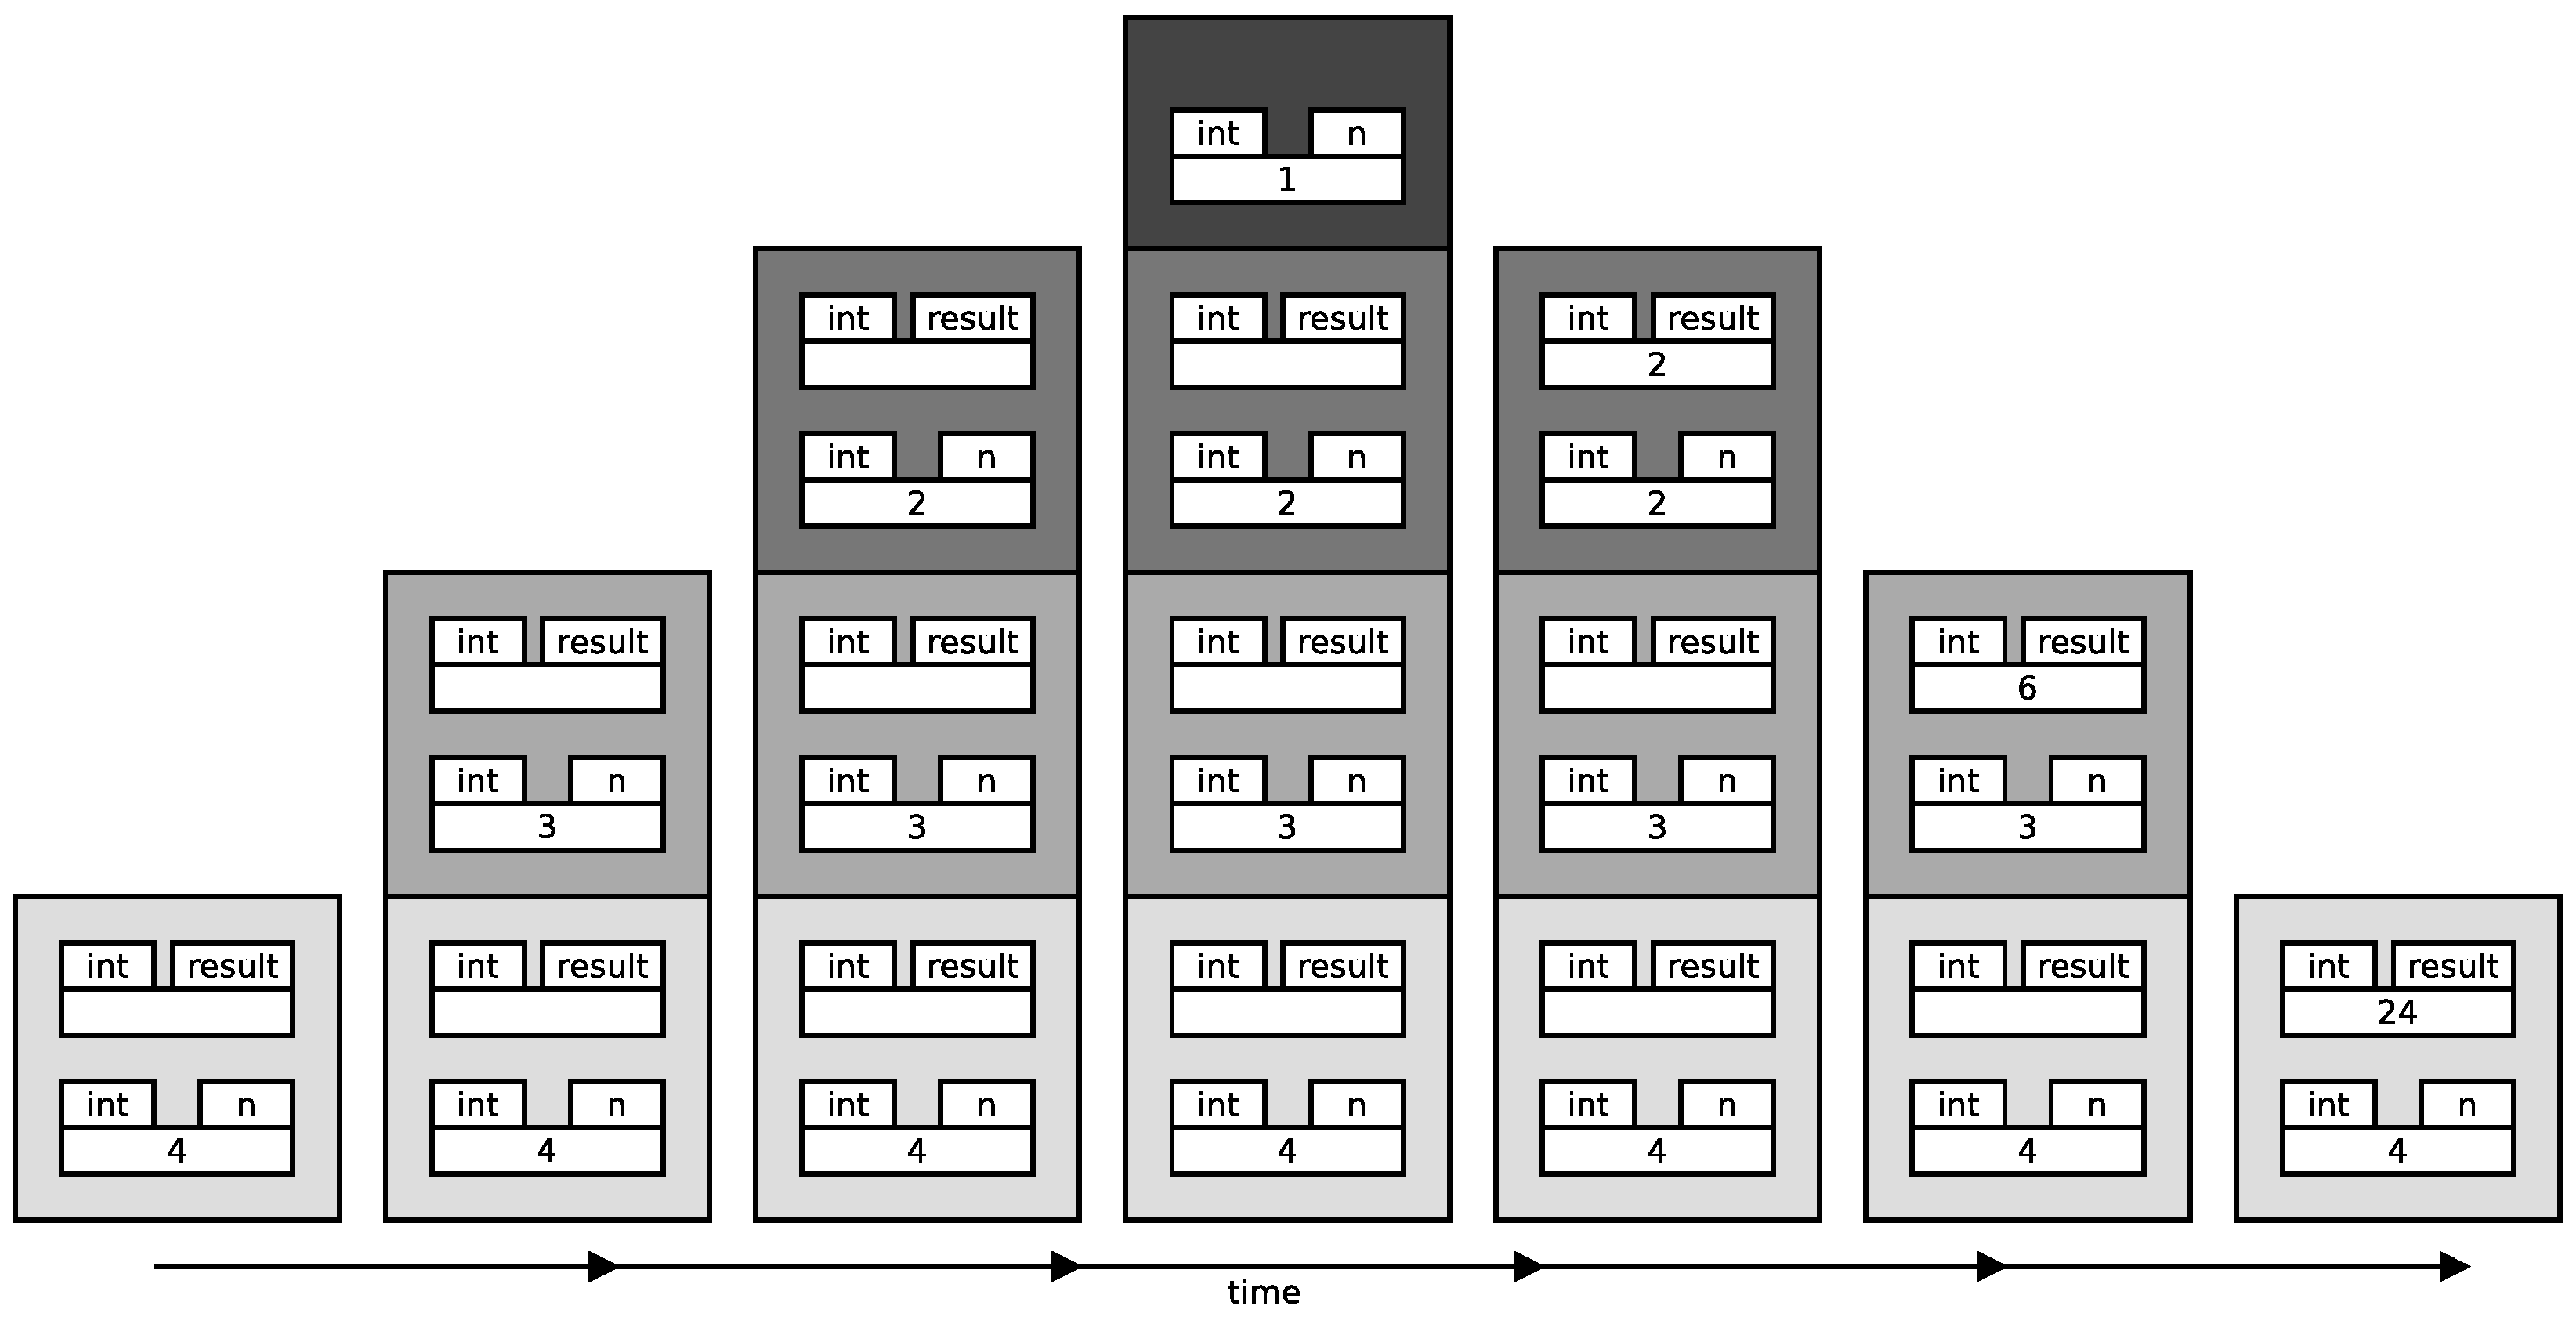
\includegraphics[width=\textwidth]{gfx/recursive-factorial}
  \caption{Evolution of the computer stack when factorial(4) is called.}
  \label{fig:fact}
\end{figure}

\subsection{Pitfalls}
\label{sec:pitfalls}

At this point you are familiar with loops (\verb+while+, \verb+for+,
\verb+do...while+) and you know that you must be careful with the
way you set the condition of a loop to prevent infinite loops that
block your programs. In a similar way, you must keep in mind a couple
of things when you write recursive code. 

\paragraph{Base case}
\label{sec:base-case}

Every recursive program or method must have a base case for which the
answer is known. In the case of the factorial, we know that~1! is~1;
in the case of the Fibonacci numbers, we know 
that the answer for F(1) and F(2) is~1; when we calculate the depth of
of a tree, we know that the depth of a tree with no descendants is 0;
when we add a new element to a a list recursively, we know that the
element will be added to the element were \verb+next+ is pointing to
\verb+null+. 

If a recursive method does not have a base case, the method will call
itself continuously until the stack is overflown, i.e.~until the
computer tries to add a new level to the stack (to execute the next
method) and find there is no more space to do it. At that point, the
Java Virtual Machine will throw a \verb+StackOverflow+ exception. 

\paragraph{No convergence}
\label{sec:no-convergence}

Apart from a base case, it is important that each iteration of a
recursive method tries to answer a simpler or more limited version of
the same question. In other words, every time a method is called again
its parameter must be a smaller number, or a shorter list, or ---in
general--- must be nearer to the base case. 

In simple cases like the factorial or the Fibonacci numbers, it is
easy to see that the method will converge. This can be more difficult
when the recursion involves more than one method, e.g.~method A calls
method B, and method B recursively calls A (A and B may be methods in
different classes\footnote{A real story: There was a project in which
  we had a window, and inside of it a canvas on which different
  objects were painted. Different elements of the application needed
  to know where the origin was; some of them asked the window and some
  of them asked the canvas. If the window did not know where the
  origin was (e.g.~at initialisation), it asked the canvas. The canvas
  set the origin at initialisation, and informed the window. If the
  user started a new canvas (e.g.~by opening a new file), the new
  canvas did not know the origin but it could as the window (which was
  already there). All was working well until the first day that a
  user, instead of starting the application and then a file, opened a
  file directly. The file opened in a canvas, that did not know where
  the origin was, so it asked the window; the window had not been told
  where the origin was, so it asked the canvas; and the recursive loop
  continued until the application crashed in front of the eyes of the
  (quite upset) user.}). You must be especially careful when you have
a loop of several methods calling each other recursively because it
may be quite complex to see whether they converge in all cases or not.

If your recursive method does not converge towards a base case, you
will overflow the stack and the Java Virtual Machine will throw a
\verb+StackOverflow+ exception. 



% Recursion
%   - takes more stack space, but usually improves legibility
%   - search for something that can only be done recursively
%     - there is no such thing, this is a consequence of the
%       Turing-Church conjecture.  
%   - when to go iterative and when to go recursive
%     - simplicity and clarity vs resources, the former win every day
%       (if they do not, they will soon)
%     - counter-example: fibonacci
%   - cpu vs memory: dynamic programming
%     - memoizing
%     - fibonacci example
%   - divide and conquer
%     - example in real life: sorting postal mail (thanks to Knuth)
%     - binary search
%     - quick sort
%     - Advantages: easier to parallelise -> will come to it again

% Exercises
%   - write numbers...  then check
%   - What is wrong with this exercise? (check for 0 is too late!)
%   - Factorial and fibonacci
%   - hanoi towers
%   - Greatest common divisor ( p > q => gcd(p,q) = gcd(q, p % q) )
%   - Anagrams of n letters
%   - adding elements / calculating length of queue
%     - Length of a queue
%   - Power of a number
%   - Koch star?
%   - Din-A4, etc
%   - merge sort
%   - Finding longest common subsequence
%   - Root finding for a polynomial (one between -1000 and 1000 if
%       sign(f(min)) != sign(f(max)) , as many as possible for **)
%   - Memoization: Collatz problem
%   - Memoization: McCarthy
%   - 8 dames on a chess board
%   - Increments and unfolding
%   - Towers of Hanoi variant: odd vs even
%   - Dominoes
%   - How big is your stack? 


%%% Local Variables:
%%% mode: latex
%%% TeX-master: "d13"
%%% End:
